\chapter{Case Study}
\todo{Describe the case study: two different steps, the first one without code modification (monitoring of existing communication channels), the second one where code is actually modified to emit special debugging messages (can be done with rosdashboards api or manually).}

\todo{Talk to Jamie Diprose about his Nao work with ROS (probably better than the turtlesim example from the ICRA paper), or see if rosbag data can be found and build showcase on top of the rosbag data.}

\section{Visualizing Existing Data}
Although the current implementation is a prototype, it has all the features that were initially planned. The implementation is running stably and first attempts to use it as a debugging tool have been made. ROSDashboard is ready to be used for the development of robot applications and can be used for further evaluations (see Section~\ref{future_work}).

Figure~\ref{showcase} shows a simple showcase scenario: ROSDashboard is running alongside the \emph{turtlesim\_node} node which is used in many examples in the ROS tutorials\footnote{http://www.ros.org/wiki/ROS/Tutorials}. It monitors the values for linear and angular speed which are published by the \emph{turtle\_teleop\_key} node to control the turtle simulation. The String widget is configured to display messages from \emph{/rosout}, which in this example shows a warning when the turtle hits a wall.
For the purpose of this small showcase, there was no need to modify the turtlesim source code. The only topics used by the showcase scenario are topics that are already used to control the turtle in the simulation and to display warnings.

\begin{figure}[thpb]
  \centering
  \framebox{
    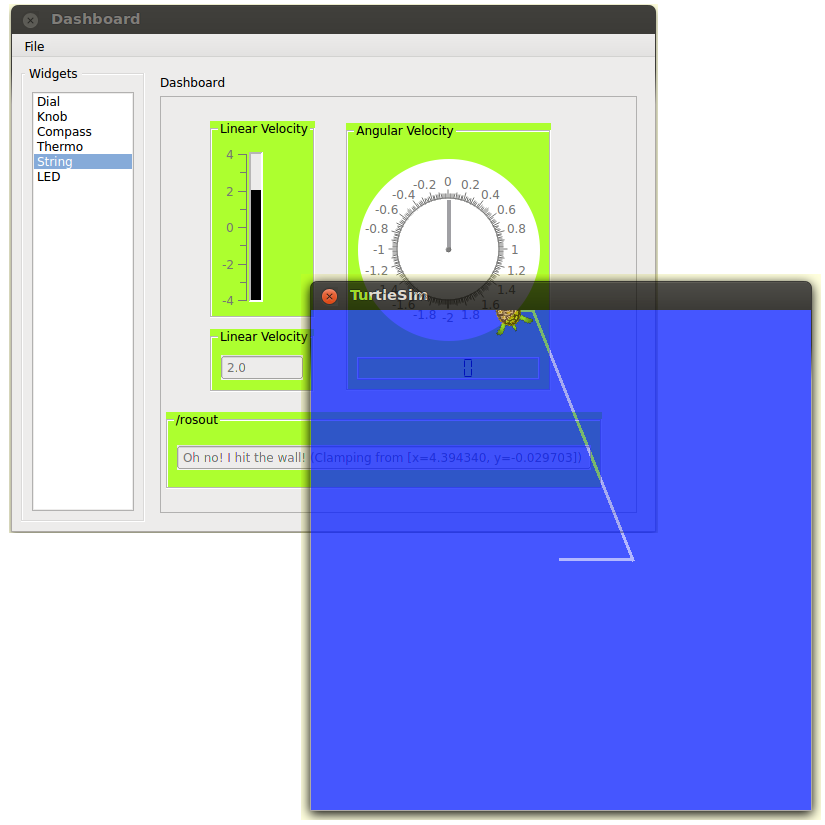
\includegraphics[width=0.9\textwidth]{img/showcase3.png}
  }  
  \caption{ROSDashboard running alongside turtlesim\_node.}
  \label{showcase}
\end{figure}

Figure~\ref{rosgraph_simple} shows the ROS computation graph during the execution of the showcase scenario. It shows how ROSDashboard is connected to the nodes which are debugged. The topics needed for the showcase are \emph{/turtle1/command\_velocity} for the linear and angular velocity and \emph{/rosout} for warnings when the turtle hit the wall.

\begin{figure}[thpb]
  \centering
  \framebox{
    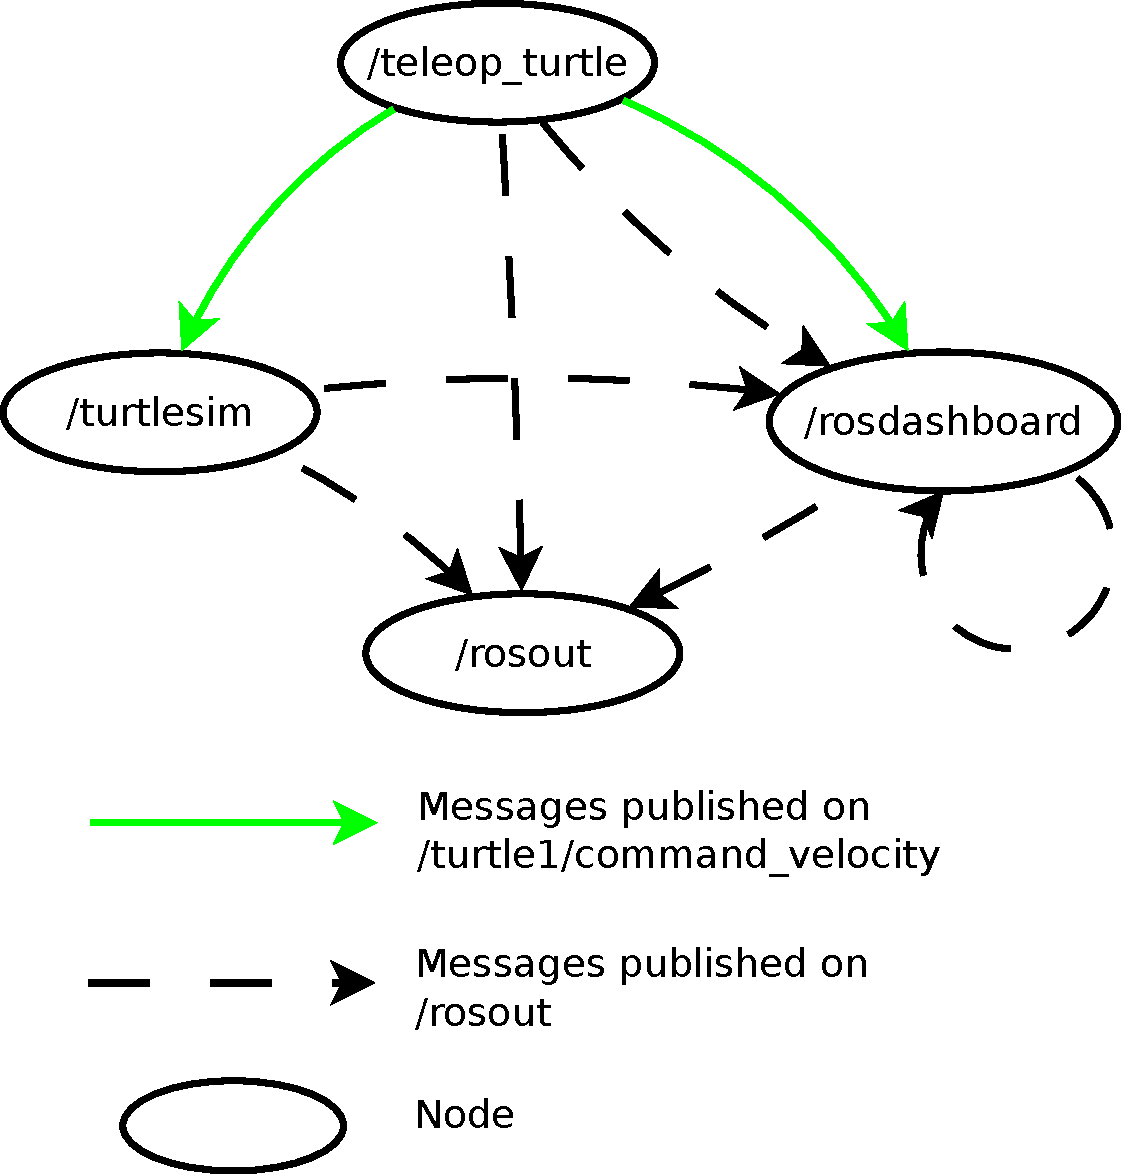
\includegraphics[width=0.7\textwidth]{diagrams/rosgraph}
  }  
  \caption{Simplified ROS computation graph with ROSDashboard.}
  \label{rosgraph_simple}
\end{figure}

\section{Adding New Widgets}
\todo{this could be a good spot for the section from the previous chapter about the plot widget}

\subsection{Case Study Configuration}
\todo{is this important? drop}
\todo{old structure}
What machines, software versions, robots, etc were used.

\subsection{Without Code Modification}
\todo{old structure}
\subsection{With Code Modification}
\todo{old structure}
\subsection{Discussion}
Discuss the results from the case study?
